\section{Experiments}
\label{sec:experiments}


% ==========================
% Table 1: Performance comparison with baseline models
% ==========================
\begin{table*}[t]
\centering
\caption{Performance comparison of SAGE with ConvNeXt and Vision Transformer UNet (SAGE-ConvNeXt+ViT-UNet) against a comprehensive suite of baseline models on EBHI and GlaS datasets. The results demonstrate that SAGE-ConvNeXt+ViT-UNet sets a new performance benchmark, surpassing the best existing backbones across all metrics. All scores are percentages (\%). \colorbox{BestColor}{\textcolor{BestTextColor}{\textbf{Best}}} and \colorbox{SecondBestColor}{\textcolor{SecondBestTextColor}{Second}} indicate the best and the second-best performance, respectively.}
\label{tab:baseline_results}

\setlength{\tabcolsep}{2pt}
% \scriptsize
\setlength{\arrayrulewidth}{0.25pt}
\resizebox{\textwidth}{!}{%
\begin{tabular}{l|ccccc|cccccc|cccccc}
\toprule
\textbf{Model} & \multicolumn{5}{c|}{\centering\textbf{EBHI}} & \multicolumn{6}{c|}{\centering\textbf{GlaS (Test A)}} & \multicolumn{6}{c}{\centering\textbf{GlaS (Test B)}} \\
 & \multicolumn{5}{c|}{\centering\textbf{(Adenocarcinoma)}} & \multicolumn{6}{c|}{\centering\textbf{ }} & \multicolumn{6}{c}{\centering\textbf{ }} \\
\cmidrule{2-6} \cmidrule{7-12} \cmidrule{13-18} 
& Acc $\uparrow$ & IoU $\uparrow$ & DSC $\uparrow$ & HD95 $\downarrow$ & B-F1 $\uparrow$ & Acc $\uparrow$ & IoU $\uparrow$ & DSC $\uparrow$ & HD95 $\downarrow$ & B-F1 $\uparrow$ & O-DSC $\uparrow$ & Acc $\uparrow$ & IoU $\uparrow$ & DSC $\uparrow$ & HD95 $\downarrow$ & B-F1 $\uparrow$ & O-DSC $\uparrow$ \\
\midrule
ResNet101-UNet \cite{ronneberger2015unetconvolutionalnetworksbiomedical, he2015deepresiduallearningimage} 
& 91.93 & 89.11 & 94.24 & 46.15 & 55.58 
& 87.52 & 77.75 & 87.49 & 32.37 & 60.11 & 41.68 
& 85.72 & 78.46 & 87.93 & 26.10 & 56.69 & 40.11 \\

ResNet152-UNet \cite{ronneberger2015unetconvolutionalnetworksbiomedical, he2015deepresiduallearningimage} 
& 91.64 & 88.69 & 94.00 & 45.93 & 54.89 
& 87.60 & 77.76 & 87.60 & 33.08 & 55.79 & 33.81 
& 84.28 & 76.73 & 86.83 & 26.14 & 49.10 & 27.69 \\

EfficientNet-B7-UNet \cite{ronneberger2015unetconvolutionalnetworksbiomedical, tan2020efficientnetrethinkingmodelscaling} 
& 91.82 & 89.00 & 94.18 & 46.37 & 54.45 
& 87.92 & 78.77 & 88.12 & 33.57 & 53.26 & 22.99 
& 84.97 & 77.14 & 87.09 & 30.26 & 51.25 & 24.33 \\

ConvNeXt-UNet \cite{ronneberger2015unetconvolutionalnetworksbiomedical, ConvNext} 
& 91.87 & 89.07 & 94.22 & 46.01 & 54.59 
& \cellcolor{SecondBestColor}\textcolor{SecondBestTextColor}{91.91} & \cellcolor{SecondBestColor}\textcolor{SecondBestTextColor}{85.03} & \cellcolor{SecondBestColor}\textcolor{SecondBestTextColor}{91.91} & \cellcolor{SecondBestColor}\textcolor{SecondBestTextColor}{23.39} & 68.03 & 54.31
& 88.22 & 81.68 & 89.91 & 25.85 & 59.37 & 49.17 \\

U-Net++ (ResNet 101) \cite{zhou2018unet++} 
& 91.94 & 89.13 & 94.25 & \cellcolor{SecondBestColor}\textcolor{SecondBestTextColor}{45.51} & 56.00 
& 89.01 & 80.40 & 89.13 & 30.21 & 61.14 & 29.21 
& 86.23 & 79.30 & 88.46 & 26.34 & 53.08 & 19.38 \\

UMamba \cite{ma2024u} 
& 91.51 & 88.55 & 93.93 & 49.79 & 51.66 
& 83.64 & 72.17 & 83.83 & 34.31 & 53.14 & 36.40 
& 84.46 & 77.22 & 87.15 & 26.23 & 54.89 & 45.00 \\

Swin UMamba \cite{liu2024swin} 
& 92.01 & 89.18 & \cellcolor{SecondBestColor}\textcolor{SecondBestTextColor}{94.28} & 48.35 & 55.23 
& 86.57 & 76.09 & 86.42 & 34.93 & 60.59 & 35.46 
& 84.00 & 75.00 & 85.72 & 26.76 & 58.29 & 38.37 \\

Swin U-Net \cite{cao2022swin} 
& 91.97 & 89.10 & 94.24 & 45.73 & 53.06 
& 90.53 & 82.72 & 90.54 & 26.89 & 60.20 & 45.20 
& 86.82 & 79.52 & 88.59 & 24.82 & 54.70 & 43.09 \\

\midrule

ResNet34-UNet \cite{ronneberger2015unetconvolutionalnetworksbiomedical, he2015deepresiduallearningimage}
& 91.72 & 88.63 & 93.88 & 47.41 & 54.67 
& 88.91 & 81.72 & 89.78 & 26.48 & 63.84 & 55.26 
& 87.46 & 80.68 & 88.92 & 24.62 & 57.38 & 49.84 \\

\textbf{SAGE-ResNet34-UNet (Ours)}
& 92.36 & \cellcolor{SecondBestColor}\textcolor{SecondBestTextColor}{89.24} & \cellcolor{SecondBestColor}\textcolor{SecondBestTextColor}{94.28} & 46.05 & \cellcolor{SecondBestColor}\textcolor{SecondBestTextColor}{56.18} 
& 90.37 & 83.34 & 91.06 & \cellcolor{SecondBestColor}\textcolor{SecondBestTextColor}{23.39} & 69.27 & 61.18 
& 89.28 & \cellcolor{SecondBestColor}\textcolor{SecondBestTextColor}{82.11} & \cellcolor{SecondBestColor}\textcolor{SecondBestTextColor}{90.41} & \cellcolor{SecondBestColor}\textcolor{SecondBestTextColor}{21.27} & 63.45 & 56.73 \\

\midrule

ConvNeXt+ViT-UNet 
& \cellcolor{SecondBestColor}\textcolor{SecondBestTextColor}{92.49} & 83.60 & 90.94 & 46.02 & 55.60 
& 91.88 & 84.91 & 91.80 & 24.25 & \cellcolor{SecondBestColor}\textcolor{SecondBestTextColor}{75.21} & \cellcolor{SecondBestColor}\textcolor{SecondBestTextColor}{65.09} 
& \cellcolor{SecondBestColor}\textcolor{SecondBestTextColor}{89.96} & 81.80 & 89.85 & 22.32 & \cellcolor{SecondBestColor}\textcolor{SecondBestTextColor}{67.57} & \cellcolor{SecondBestColor}\textcolor{SecondBestTextColor}{59.93} \\


\textbf{SAGE-ConvNeXt+ViT-UNet (Ours)} 
& \cellcolor{BestColor}\textcolor{BestTextColor}{94.03} & \cellcolor{BestColor}\textcolor{BestTextColor}{90.90} & \cellcolor{BestColor}\textcolor{BestTextColor}{95.23} & \cellcolor{BestColor}\textcolor{BestTextColor}{45.20} & \cellcolor{BestColor}\textcolor{BestTextColor}{58.10} 
& \cellcolor{BestColor}\textcolor{BestTextColor}{92.96} & \cellcolor{BestColor}\textcolor{BestTextColor}{86.62} & \cellcolor{BestColor}\textcolor{BestTextColor}{92.78} & \cellcolor{BestColor}\textcolor{BestTextColor}{19.85} & \cellcolor{BestColor}\textcolor{BestTextColor}{77.91} & \cellcolor{BestColor}\textcolor{BestTextColor}{73.49} 
& \cellcolor{BestColor}\textcolor{BestTextColor}{91.55} & \cellcolor{BestColor}\textcolor{BestTextColor}{84.56} & \cellcolor{BestColor}\textcolor{BestTextColor}{91.42} & \cellcolor{BestColor}\textcolor{BestTextColor}{17.94} & \cellcolor{BestColor}\textcolor{BestTextColor}{70.23} & \cellcolor{BestColor}\textcolor{BestTextColor}{66.67} \\
\bottomrule
\end{tabular}
}%
\setlength{\tabcolsep}{6pt}
\setlength{\arrayrulewidth}{0.4pt}
\end{table*}



\begin{table*}[t]
\centering
\caption{Performance comparison of SAGE-ConvNeXt+ViT-UNet against leading SOTA models on EBHI and GlaS datasets. Our approach achieves a new SOTA by securing top performance across all metrics, showcasing its strong generalization to varied tissue morphologies. All metrics are reported in percentages (\%). \colorbox{BestColor}{\textcolor{BestTextColor}{\textbf{Best}}} and \colorbox{SecondBestColor}{\textcolor{SecondBestTextColor}{Second}} indicate the best and the second-best performance, respectively.}
\label{tab:sota_results}
\setlength{\tabcolsep}{2pt}
\scriptsize
\setlength{\arrayrulewidth}{0.25pt}
\resizebox{\textwidth}{!}{%
\begin{tabular}{l|ccccc|cccccc|cccccc}
\toprule
\textbf{Model} & \multicolumn{5}{c|}{\centering\textbf{EBHI}} & \multicolumn{6}{c|}{\centering\textbf{GlaS (Test A)}} & \multicolumn{6}{c}{\centering\textbf{GlaS (Test B)}} \\
 & \multicolumn{5}{c|}{\centering\textbf{(Adenocarcinoma)}} & \multicolumn{6}{c|}{\centering\textbf{ }} & \multicolumn{6}{c}{\centering\textbf{ }} \\
\cmidrule{2-6} \cmidrule{7-12} \cmidrule{13-18} 
& Acc $\uparrow$ & IoU $\uparrow$ & DSC $\uparrow$ & HD95 $\downarrow$ & B-F1 $\uparrow$ & Acc $\uparrow$ & IoU $\uparrow$ & DSC $\uparrow$ & HD95 $\downarrow$ & B-F1 $\uparrow$ & O-DSC $\uparrow$ & Acc $\uparrow$ & IoU $\uparrow$ & DSC $\uparrow$ & HD95 $\downarrow$ & B-F1 $\uparrow$ & O-DSC $\uparrow$ \\

\midrule
SelfReg-UNet \cite{zhu2024selfreg} 
& 91.53 & 88.58 & 93.95 & 45.66 & 53.83 
& 89.36 & 80.34 & 89.10 & 28.57 & 65.82 & 47.17 
& 86.21 & 77.93 & 87.60 & 26.33 & 59.95 & 40.16 \\

Attention U-Net \cite{oktay2018attention} 
& 92.11 & 89.28 & 94.34 & 46.43 & 57.64 
& 90.53 & 82.43 & 90.37 & 65.60 & 45.95 & 59.03 
& 87.57 & 80.29 & 89.07 & 56.51 & 38.87 & 54.77 \\

ConvUNeXt \cite{han2022convunext} 
& 90.73 & 87.66 & 93.43 & 47.93 & 49.86 
& 87.68 & 77.61 & 87.39 & 28.70 & 62.80 & 45.60 
& 88.05 & 81.16 & 89.60 & \cellcolor{SecondBestColor}\textcolor{SecondBestTextColor}{20.46} & 60.58 & 42.96 \\

UCTransNet \cite{wang2022uctransnet} 
& 91.95 & 89.07 & 94.22 & 46.67 & 57.22 
& 87.07 & 76.47 & 86.66 & 29.23 & 62.97 & 49.38 
& 85.45 & 77.14 & 87.10 & 26.66 & 58.51 & 58.00 \\

TransAttUNet \cite{chen2023transattunet} 
& 91.40 & 88.52 & 93.91 & 50.02 & 51.40 
& 91.18 & 83.69 & 91.12 & 24.51 & 72.13 & 66.65 
& \cellcolor{SecondBestColor}\textcolor{SecondBestTextColor}{89.87} & \cellcolor{SecondBestColor}\textcolor{SecondBestTextColor}{83.78} & \cellcolor{SecondBestColor}\textcolor{SecondBestTextColor}{91.18} & 22.41 & 64.27 & 60.86 \\

SegFormer \cite{xie2021segformer}
& 92.62 & 89.93 & 94.70 & \cellcolor{BestColor}\textcolor{BestTextColor}{42.43} & 55.16 
& 91.09 & 83.31 & 90.89 & \cellcolor{SecondBestColor}\textcolor{SecondBestTextColor}{20.72} & 61.65 & 53.72 
& 87.47 & 80.45 & 89.16 & 23.60 & 55.95 & 51.54 \\

EViT-UNet \cite{li2025evit} 
& \cellcolor{SecondBestColor}\textcolor{SecondBestTextColor}{92.80} & \cellcolor{SecondBestColor}\textcolor{SecondBestTextColor}{90.23} & \cellcolor{SecondBestColor}\textcolor{SecondBestTextColor}{94.86} & 45.30 & \cellcolor{BestColor}\textcolor{BestTextColor}{59.99} 
& \cellcolor{SecondBestColor}\textcolor{SecondBestTextColor}{92.70} & \cellcolor{SecondBestColor}\textcolor{SecondBestTextColor}{86.15} & \cellcolor{SecondBestColor}\textcolor{SecondBestTextColor}{92.56} & 21.82 & \cellcolor{SecondBestColor}\textcolor{SecondBestTextColor}{76.54} & \cellcolor{SecondBestColor}\textcolor{SecondBestTextColor}{73.26} 
& 89.61 & 83.62 & 91.08 & 21.24 & \cellcolor{SecondBestColor}\textcolor{SecondBestTextColor}{65.62} & 63.24 \\

CAC-UNet \cite{zhu2021multi} 
& 91.32 & 88.40 & 93.84 & 51.35 & 53.42 
& 88.01 & 78.34 & 87.85 & 31.70 & 64.29 & 53.81 
& 85.69 & 77.52 & 87.33 & 27.87 & 58.11 & 46.02 \\

TransUNet \cite{chen2021transunet} 
& 91.46 & 88.38 & 93.83 & 45.76 & 53.96 
& 91.26 & 83.72 & 91.14 & 23.46 & 63.62 & 67.33 
& 87.30 & 79.98 & 88.87 & 22.77 & 55.63 & \cellcolor{SecondBestColor}\textcolor{SecondBestTextColor}{63.56} \\

\midrule
\textbf{SAGE-ConvNeXt+ViT-UNet (Ours)} 
& \cellcolor{BestColor}\textcolor{BestTextColor}{94.03} & \cellcolor{BestColor}\textcolor{BestTextColor}{90.90} & \cellcolor{BestColor}\textcolor{BestTextColor}{95.23} & \cellcolor{SecondBestColor}\textcolor{SecondBestTextColor}{45.20} & \cellcolor{SecondBestColor}\textcolor{SecondBestTextColor}{58.10} 
& \cellcolor{BestColor}\textcolor{BestTextColor}{92.96} & \cellcolor{BestColor}\textcolor{BestTextColor}{86.62} & \cellcolor{BestColor}\textcolor{BestTextColor}{92.78} & \cellcolor{BestColor}\textcolor{BestTextColor}{19.85} & \cellcolor{BestColor}\textcolor{BestTextColor}{77.91} & \cellcolor{BestColor}\textcolor{BestTextColor}{73.49} 
& \cellcolor{BestColor}\textcolor{BestTextColor}{91.55} & \cellcolor{BestColor}\textcolor{BestTextColor}{84.56} & \cellcolor{BestColor}\textcolor{BestTextColor}{91.42} & \cellcolor{BestColor}\textcolor{BestTextColor}{17.94} & \cellcolor{BestColor}\textcolor{BestTextColor}{70.23} & \cellcolor{BestColor}\textcolor{BestTextColor}{66.67} \\
\bottomrule
\end{tabular}
}%
\setlength{\tabcolsep}{6pt}
\setlength{\arrayrulewidth}{0.4pt}
\end{table*}



% ==========================
% Table 3: Performance comparison with SOTA models on DigestPath
% ==========================
\begin{table}[t]
\centering
\caption{Performance comparison of SAGE-ConvNeXt+ViT-UNet against leading SOTA models on the DigestPath dataset. The results are evaluated across both Patch and WSI levels. All metrics are reported in percentages (\%). \colorbox{BestColor}{\textcolor{BestTextColor}{\textbf{Best}}} and \colorbox{SecondBestColor}{\textcolor{SecondBestTextColor}{Second}} indicate the best and the second-best performance among all models, respectively.}
\label{tab:digestpath_sota_results}

\setlength{\tabcolsep}{2pt}
\scriptsize
\setlength{\arrayrulewidth}{0.25pt}
\resizebox{\columnwidth}{!}{%
\begin{tabular}{l|ccccc|ccccc}
\toprule
\textbf{Model} & \multicolumn{10}{c}{\centering\textbf{DigestPath}} \\
\cmidrule{2-11}
& \multicolumn{5}{c|}{\centering\textbf{Patch}} & \multicolumn{5}{c}{\centering\textbf{WSI}} \\
\cmidrule{2-6} \cmidrule{7-11}
& Acc $\uparrow$ & IoU $\uparrow$ & DSC $\uparrow$ & HD95 $\downarrow$ & B-F1 $\uparrow$ & Acc $\uparrow$ & IoU $\uparrow$ & DSC $\uparrow$ & HD95 $\downarrow$ & B-F1 $\uparrow$ \\
\midrule
SelfReg-UNet \cite{zhu2024selfreg}
& 96.28 & 80.05 & 83.32 & 131.20 & 71.61
& 97.77 & 78.06 & 83.04 & 417.45 & 60.09 \\

Attention U-Net \cite{oktay2018attention}
& 96.81 & 80.47 & 83.97 & 123.71 & 72.29
& \cellcolor{SecondBestColor}\textcolor{SecondBestTextColor}{98.03} & 80.30 & 85.36 & 416.23 & 61.31 \\

ConvUNeXt \cite{han2022convunext}
& 96.84 & 77.71 & 81.22 & 123.98 & 69.40
& \cellcolor{SecondBestColor}\textcolor{SecondBestTextColor}{98.03} & 74.20 & 79.25 & 576.06 & 55.37 \\

UCTransNet \cite{wang2022uctransnet}
& 96.63 & 81.54 & 84.89 & 121.27 & 73.81
& 97.95 & 84.44 & 89.44 & 427.20 & 66.35 \\

TransAttUNet \cite{chen2023transattunet}
& 96.86 & 80.37 & 83.69 & 126.87 & 71.37
& 98.02 & 75.53 & 80.45 & 454.48 & 56.00 \\

SegFormer \cite{xie2021segformer}
& \cellcolor{SecondBestColor}\textcolor{SecondBestTextColor}{96.99} & 84.54 & 87.66 & 115.75 & 76.54
& 97.97 & \cellcolor{SecondBestColor}\textcolor{SecondBestTextColor}{85.51} & \cellcolor{SecondBestColor}\textcolor{SecondBestTextColor}{90.56} & 393.11 & \cellcolor{SecondBestColor}\textcolor{SecondBestTextColor}{67.15} \\

EViT-UNet \cite{li2025evit}
& 96.60 & 83.38 & 86.37 & 120.47 & 76.38
& 98.02 & 83.16 & 87.78 & \cellcolor{SecondBestColor}\textcolor{SecondBestTextColor}{364.86} & 65.97 \\

CAC-UNet \cite{zhu2021multi}
& 96.81 & 81.74 & 84.99 & \cellcolor{SecondBestColor}\textcolor{SecondBestTextColor}{61.10} & \cellcolor{SecondBestColor}\textcolor{SecondBestTextColor}{78.78}
& 97.96 & 83.63 & 88.66 & 528.06 & 65.03 \\

TransUNet \cite{chen2021transunet}
& 96.79 & 83.19 & 86.50 & 119.96 & 74.40
& 97.92 & 82.25 & 87.28 & 419.77 & 63.18 \\

\midrule

ConvNeXt+ViT-UNet
& 96.80 & \cellcolor{SecondBestColor}\textcolor{SecondBestTextColor}{89.51} & \cellcolor{SecondBestColor}\textcolor{SecondBestTextColor}{91.96} & 132.88 & 75.91
& 97.95 & 83.46 & 88.69 & 482.08 & 65.16 \\

\textbf{SAGE-ConvNeXt+ViT-UNet (Ours)}
& \cellcolor{BestColor}\textcolor{BestTextColor}{97.69} & \cellcolor{BestColor}\textcolor{BestTextColor}{90.21} & \cellcolor{BestColor}\textcolor{BestTextColor}{92.66} & \cellcolor{BestColor}\textcolor{BestTextColor}{60.67} & \cellcolor{BestColor}\textcolor{BestTextColor}{79.48}
& \cellcolor{BestColor}\textcolor{BestTextColor}{98.73} & \cellcolor{BestColor}\textcolor{BestTextColor}{86.21} & \cellcolor{BestColor}\textcolor{BestTextColor}{91.26} & \cellcolor{BestColor}\textcolor{BestTextColor}{362.31} & \cellcolor{BestColor}\textcolor{BestTextColor}{67.85} \\
\bottomrule
\end{tabular}
}%
\setlength{\tabcolsep}{6pt}
\setlength{\arrayrulewidth}{0.4pt}
\end{table}


\vspace{-0.2em}
\begin{figure}[t]
    \centering
    % --- fine-tuned layout ---
    \setlength{\tabcolsep}{1.2pt} % giảm khoảng cách giữa các cột
    \renewcommand{\arraystretch}{0.91}

    % mỗi hình chiếm ~0.1 textwidth; tổng 5 cột ~0.48 textwidth
    \newcommand{\imgw}{0.138\textwidth}
    \newcommand{\stackvsep}{0.4mm}

    \resizebox{\linewidth}{!}{%
\begin{tabular}{@{}p{0.015\textwidth}cccc@{}}
        & \scriptsize\textbf{(a) Input} &
        \scriptsize\textbf{(b) TransUNet} &
        \scriptsize\textbf{(c) EViT-UNet} &
        \scriptsize\textbf{(d) Ours} \\[2pt]

        % ============ GlaS Test A ============
        \raisebox{-0.5\totalheight}{\rotatebox{90}{\scriptsize\textbf{GlaS Test A}}} &
        \begin{minipage}{\imgw}
            
\includegraphics[width=\linewidth]{figs/testA_org_img.png}\\[-\stackvsep]
            
\includegraphics[width=\linewidth]{figs/testA_gt.png}
        \end{minipage} &
        \begin{minipage}{\imgw}
            
\includegraphics[width=\linewidth]{figs/testA_overlay_transunet.png}\\[-\stackvsep]
            
\includegraphics[width=\linewidth]{figs/testA_pred_transunet.png}
        \end{minipage} &
        \begin{minipage}{\imgw}
            
\includegraphics[width=\linewidth]{figs/testA_overlay_evit.png}\\[-\stackvsep]
            
\includegraphics[width=\linewidth]{figs/testA_pred_evit.png}
        \end{minipage} &
        \begin{minipage}{\imgw}
            
\includegraphics[width=\linewidth]{figs/testA_overlay_sage.png}\\[-\stackvsep]
            
\includegraphics[width=\linewidth]{figs/testA_pred_sage.png}
        \end{minipage} \\[2pt]

        % ============ GlaS Test B ============
        \raisebox{-0.5\totalheight}{\rotatebox{90}{\scriptsize\textbf{GlaS Test B}}} &
        \begin{minipage}{\imgw}
            
\includegraphics[width=\linewidth]{figs/testB_org_img.png}\\[-\stackvsep]
            
\includegraphics[width=\linewidth]{figs/testB_gt.png}
        \end{minipage} &
        \begin{minipage}{\imgw}
            
\includegraphics[width=\linewidth]{figs/testB_overlay_transunet.png}\\[-\stackvsep]
            
\includegraphics[width=\linewidth]{figs/testB_pred_transunet.png}
        \end{minipage} &
        \begin{minipage}{\imgw}
            
\includegraphics[width=\linewidth]{figs/testB_overlay_evit.png}\\[-\stackvsep]
            
\includegraphics[width=\linewidth]{figs/testB_pred_evit.png}
        \end{minipage} &
        \begin{minipage}{\imgw}
            
\includegraphics[width=\linewidth]{figs/testB_overlay_sage.png}\\[-\stackvsep]
            
\includegraphics[width=\linewidth]{figs/testB_pred_sage.png}
        \end{minipage}
    \end{tabular}%
}

    \caption{\small
        \textbf{Qualitative comparison on GlaS test samples.}
        Each column shows (a) the input image with ground-truth annotation, (b) TransUNet, (c) EViT-UNet, and (d) our proposed SAGE-ConvNeXt+ViT-UNet. 
        The top row presents a typical gland structure (GlaS Test A), while the bottom row depicts a challenging case with irregular morphology (GlaS Test B). 
        Green areas denote correct predictions, and red areas denote errors.}
    \label{fig:qualitative_results}
\end{figure}


\begin{figure}[t!]
\centering

% ================= Spacing Setup =================
\newcommand{\gap}{1pt}              % Internal vertical gap
\setlength{\tabcolsep}{1pt}         % Horizontal gap between columns
\renewcommand{\arraystretch}{1}

\newcommand{\imgw}{0.23\textwidth} % Adjusted from 0.18 to 0.23 to better fill the page width with 4 columns

\resizebox{\linewidth}{!}{%
\begin{tabular}{@{}p{0.02\textwidth}cccc@{}}
    & \scriptsize\textbf{(a) Input} &
    \scriptsize\textbf{(b) SegFormer} &
    \scriptsize\textbf{(c) EViT-UNet} &
    \scriptsize\textbf{(d) Ours} \\[4pt]

    % ================= WSI Sample 1 =================
    \raisebox{-0.5\totalheight}{\rotatebox{90}{\scriptsize\textbf{WSI Sample 1}}} &
    \begin{minipage}{\imgw}
        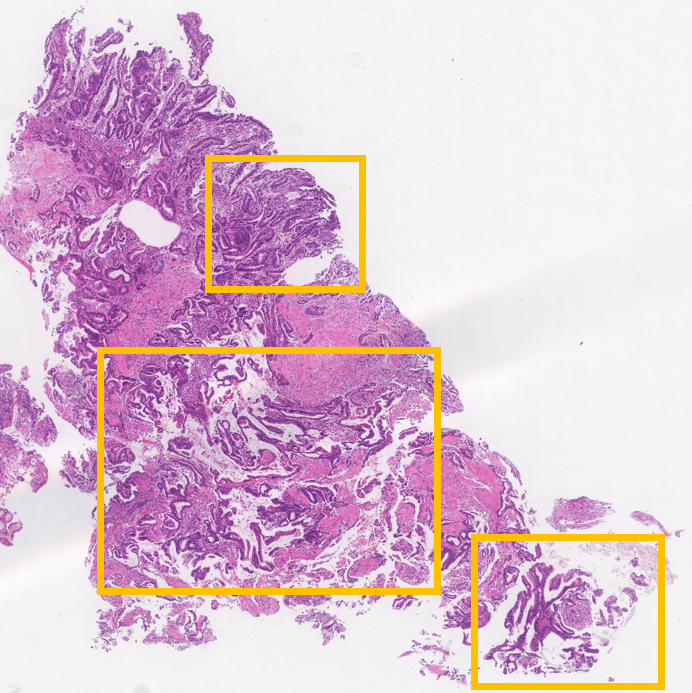
\includegraphics[width=\linewidth]{figs/wsi_img1.png}\\[\gap]
        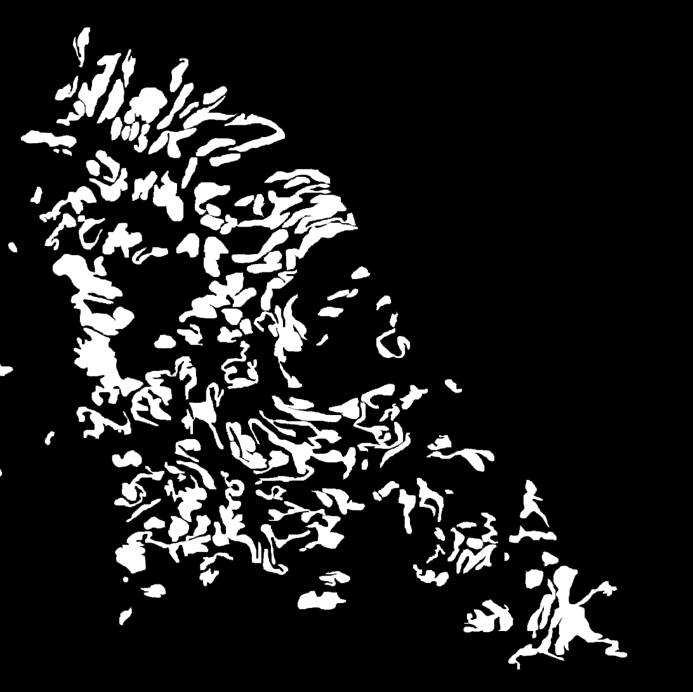
\includegraphics[width=\linewidth]{figs/wsi_gt1.png}
    \end{minipage} &
    \begin{minipage}{\imgw}
        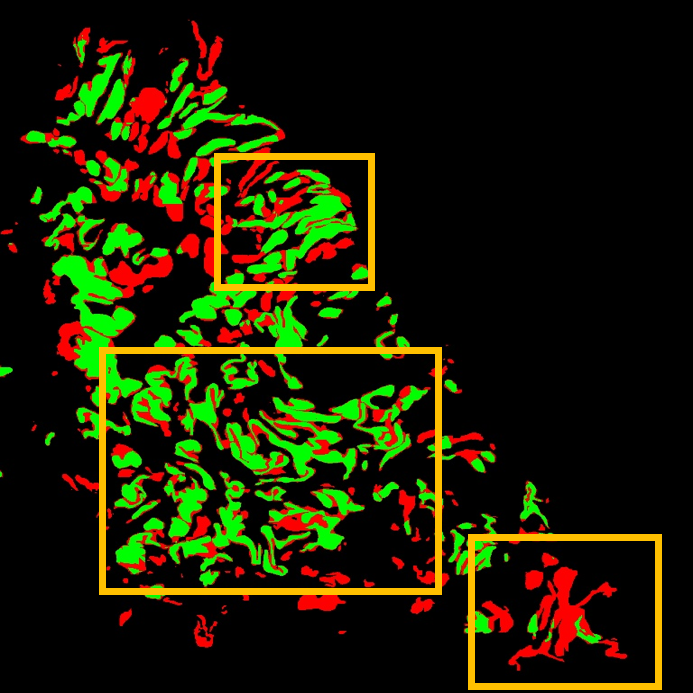
\includegraphics[width=\linewidth]{figs/segformer_wsi_overlay1.png}\\[\gap]
        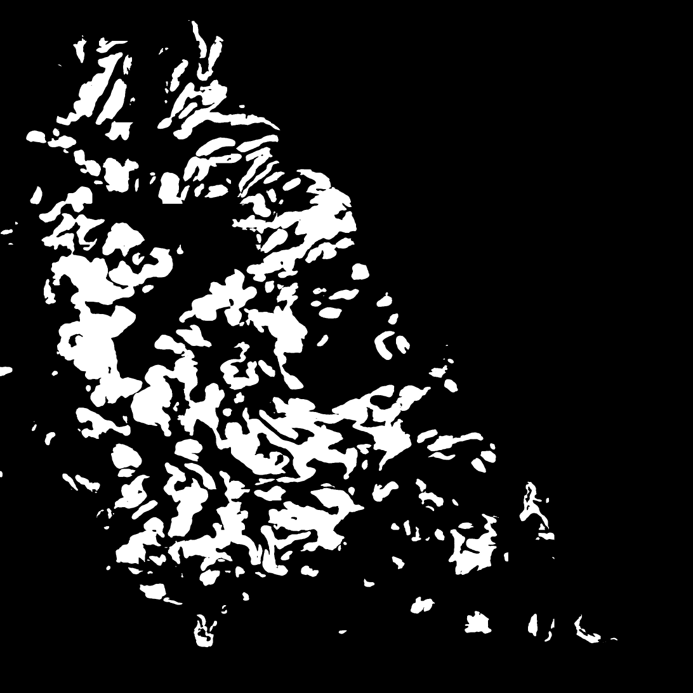
\includegraphics[width=\linewidth]{figs/segformer_wsi_pred1.png}
    \end{minipage} &
    \begin{minipage}{\imgw}
        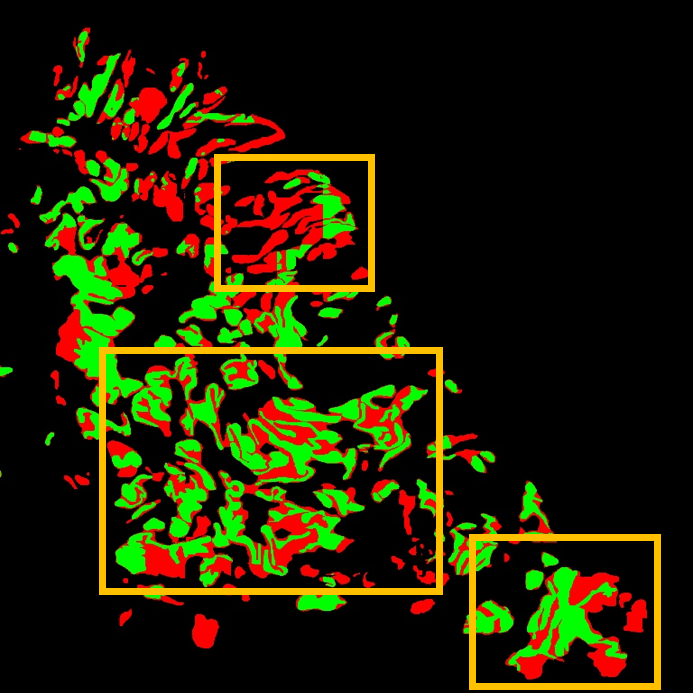
\includegraphics[width=\linewidth]{figs/evit_wsi_overlay1.png}\\[\gap]
        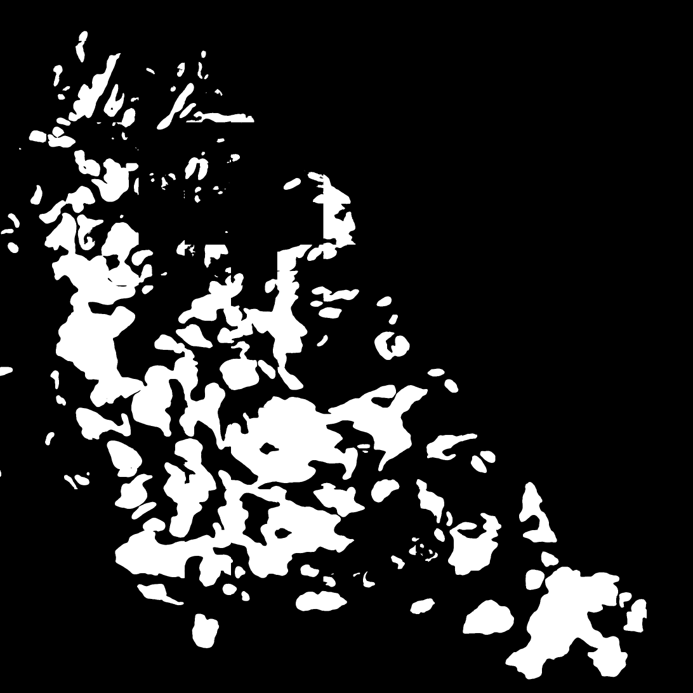
\includegraphics[width=\linewidth]{figs/evit_wsi_pred1.png}
    \end{minipage} &
    \begin{minipage}{\imgw}
        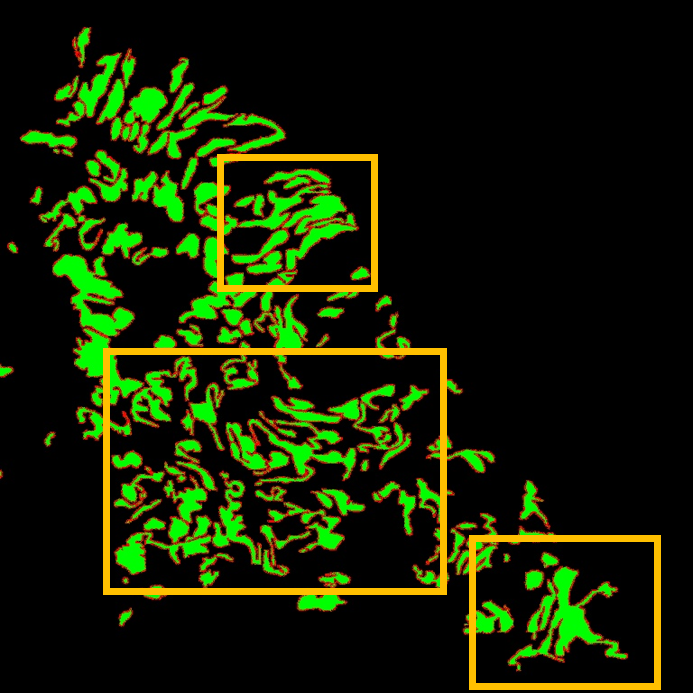
\includegraphics[width=\linewidth]{figs/sage_wsi_overlay1.png}\\[\gap]
        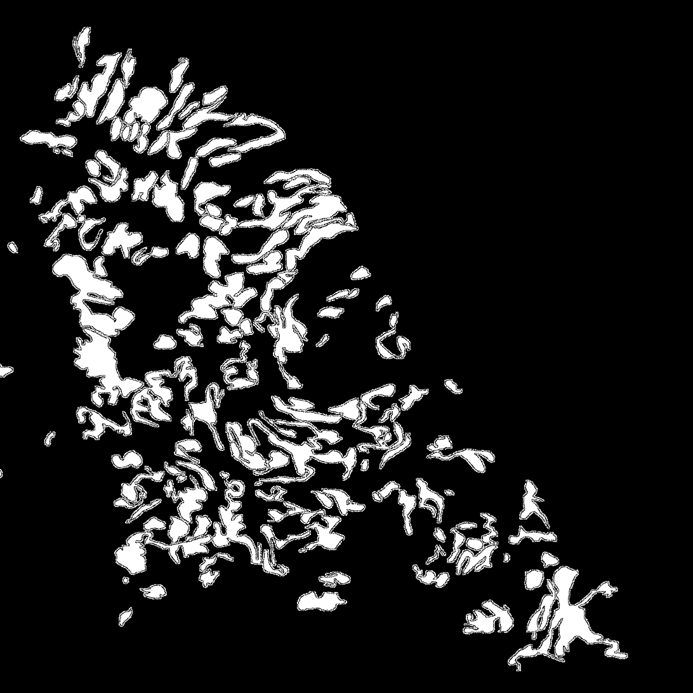
\includegraphics[width=\linewidth]{figs/sage_wsi_pred1.png}
    \end{minipage} \\
    \noalign{\vspace{2pt}}   % compact gap between Sample 1 and 2

    % ================= WSI Sample 2 =================
    \raisebox{-0.5\totalheight}{\rotatebox{90}{\scriptsize\textbf{WSI Sample 2}}} &
    \begin{minipage}{\imgw}
        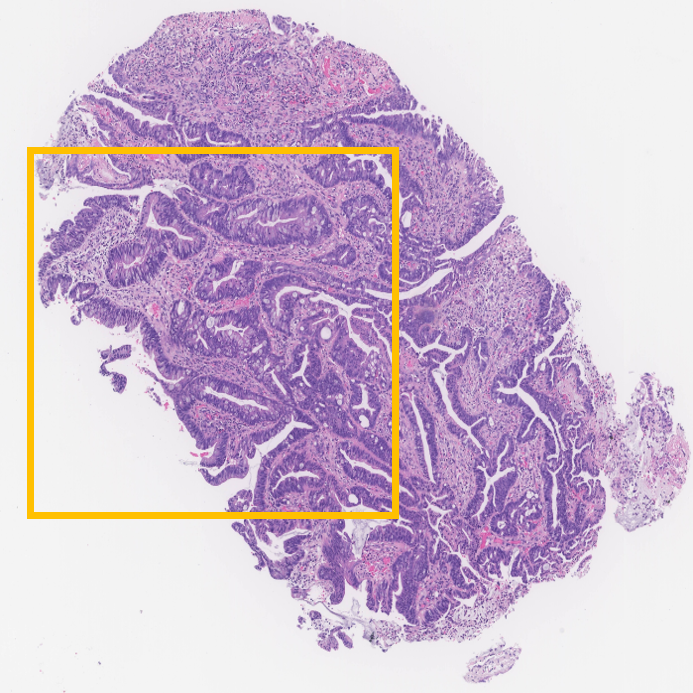
\includegraphics[width=\linewidth]{figs/wsi_img2.png}\\[\gap]
        
\includegraphics[width=\linewidth]{figs/wsi_gt2.png}
    \end{minipage} &
    \begin{minipage}{\imgw}
        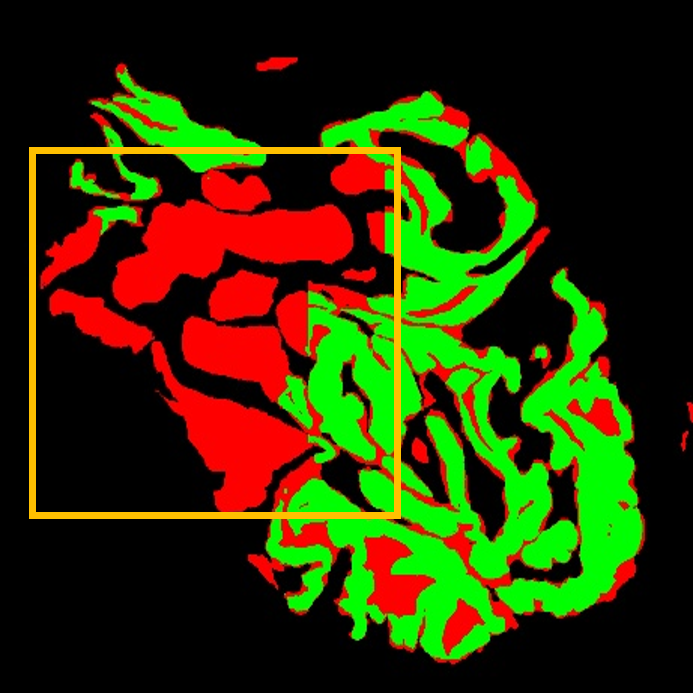
\includegraphics[width=\linewidth]{figs/segformer_wsi_overlay2.png}\\[\gap]
        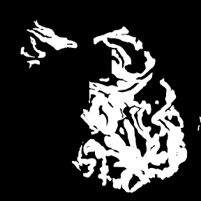
\includegraphics[width=\linewidth]{figs/segformer_wsi_pred2.png}
    \end{minipage} &
    \begin{minipage}{\imgw}
        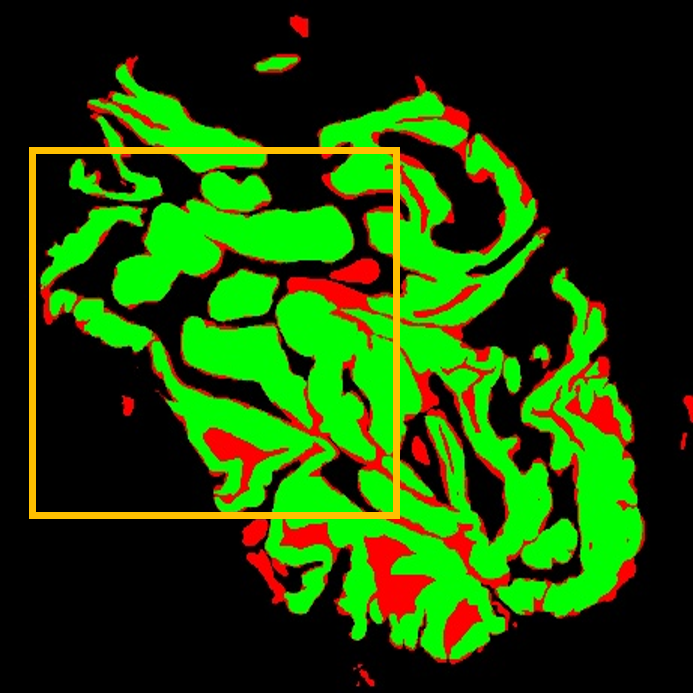
\includegraphics[width=\linewidth]{figs/evit_wsi_overlay2.png}\\[\gap]
        
\includegraphics[width=\linewidth]{figs/evit_wsi_pred2.png}
    \end{minipage} &
    \begin{minipage}{\imgw}
        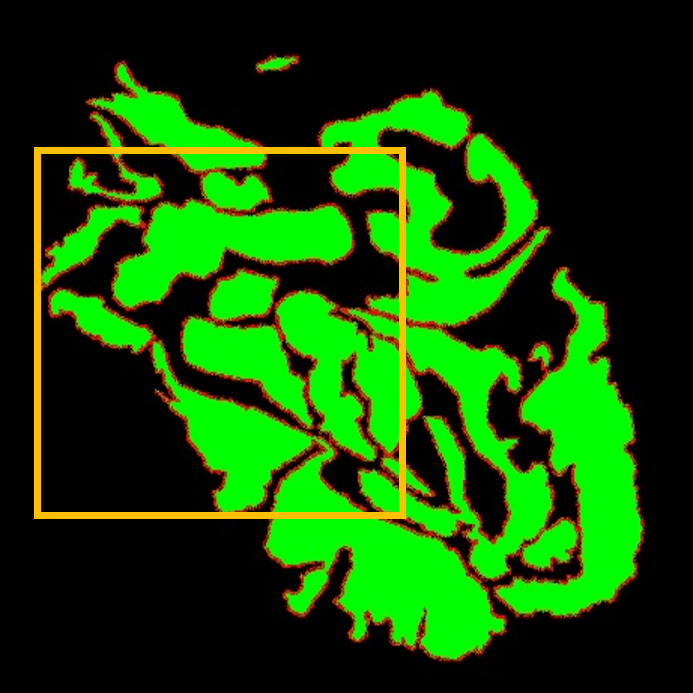
\includegraphics[width=\linewidth]{figs/sage_wsi_overlay2.png}\\[\gap]
        
\includegraphics[width=\linewidth]{figs/sage_wsi_pred2.png}
    \end{minipage} \\

\end{tabular}%
}

\caption{\small
    \textbf{Qualitative comparison on Digestpath WSI test samples.}
    Each column displays vertically stacked pairs of (a) the input image and ground-truth annotation, followed by the error overlays and binary predictions for (b) SegFormer, (c) EViT-UNet, and (d) our proposed SAGE-ConvNeXt+ViT-UNet. WSI Sample 1 (top rows) presents branching tissue structures requiring fine local boundary delineation, while WSI Sample 2 (bottom rows) depicts a dense, uniform tissue mass prone to patch-level attention collapse in pure transformer architectures. Green areas denote correct predictions, and red areas denote errors.}
\label{fig:qualitative_results_colon}

\end{figure}


\subsection{Datasets and Evaluation Metrics}
\label{subsec:datasets}
We rigorously evaluated the SAGE framework using three established public benchmarks for colorectal histopathology segmentation: \textit{EBHI},  \textit{GlaS}, and \textit{DigestPath}. 


% \vspace{0.03in}

\noindent\textbf{EBHI Dataset.}
The Extended Biopsy Histopathological Image (EBHI) dataset\cite{HU2023102534} contains $5,170$ H\&E-stained biopsy samples, each classified into one of six histological subtypes. We focused on the clinically significant \textit{Adenocarcinoma} subset, and selected $795$ images for our experiments. This dataset evaluates SAGE on heterogeneous yet domain-consistent tissue patterns.

% \vspace{0.03in}

\noindent\textbf{GlaS Dataset.} 
The Gland Segmentation (GlaS) dataset~\cite{sirinukunwattana2016glandsegmentationcolonhistology} was introduced in the MICCAI $2015$ Gland Segmentation Challenge. It consists of $165$ H\&E-stained histology images at a resolution of $522 \times 775$, each annotated for glandular structures. The official split includes $85$ images for \textit{Train}, $60$ for \textit{Test A}, and $20$ for \textit{Test B}. This dataset is widely used to assess a model's ability to capture gland morphology and boundary precision.

% \vspace{0.1in}

\noindent\textbf{DigestPath Dataset.}
The DigestPath dataset~\cite{DA2022102485} was introduced in the DigestPath $2019$ Challenge and contains $660$ gigapixel whole-slide images (WSIs) from colonoscopy specimens. To facilitate efficient training, we devised a preprocessing pipeline applied to all WSIs. Each WSI was partitioned into overlapping tiles of size $1536 \times 1536$ with stride $512$. A patch $P$ was retained only when both conditions were satisfied on its grayscale intensities:
\begin{equation*}
    P \text{ is retained iff } % iff = if and only if
\begin{cases}
\sigma(P) \ge 10, \\
\mu(P) \le 230,
\end{cases}
\end{equation*}
where $\sigma(P)$ and $\mu(P)$ denote the standard deviation and mean intensity of $P$, respectively.
This preprocessing yielded approximately $40{,}000$ patches across all WSIs, filtering out low-information background while preserving diagnostically relevant tissue regions.


% \vspace{0.1in}
\noindent\textbf{Evaluation Metrics.}
We assessed segmentation performance using a comprehensive set of metrics: pixel-wise Accuracy (ACC), Intersection over Union (IoU), Dice Similarity Coefficient (DSC), 95\% Hausdorff Distance (HD95), and Boundary F1 (B-F1). For GlaS, given its focus on object-level segmentation rather than semantic segmentation, we additionally reported the Object DSC score (O-DSC).
ACC/IoU/DSC/B-F1/O-DSC are reported in percentage (\%), while HD95 is reported in pixels.
For EBHI and GlaS, metrics are computed per image and averaged over the held-out test set.
For DigestPath, we report both patch-level and WSI-level results.
To reconstruct WSI-level predictions, overlapping patch logits are mapped back to their original slide coordinates and merged by averaging in overlap regions, followed by a threshold of $0.5$ to obtain the final binary mask; this reconstruction uses the same tiling stride ($512$) as preprocessing.


\subsection{Implementation Details}
\label{subsec:implementation}

% \vspace{0.1in}

\noindent\textbf{SAGE-ConvNeXt+ViT-UNet Configuration.}
The SAGE module was integrated into the hybrid encoder combining ConvNeXt \cite{ConvNext} and an ImageNet-pretrained ViT \cite{dosovitskiy2021imageworth16x16words}. The MoE module included $4$ shared experts and $16$ non-shared experts, with the top $4$ experts dynamically selected during routing. We trained SAGE-ConvNeXt+ViT-UNet on two NVIDIA H100 GPUs ($80$GB VRAM each) with a global batch size of $64$ ($32$ per GPU). Training proceeded in two stages using the AdamW optimizer \cite{loshchilov2019decoupledweightdecayregularization} and the hybrid loss $\mathcal{L}_{\text{total}}$ in Algorithm~\ref{alg:sage}, weighted as $\lambda_{\text{ce}} = 1$, $\lambda_{\text{dice}} = 1.5$, $\lambda_{\text{lb}} = 1$. In the first stage, all parameters were optimized with a uniform learning rate of $1\times10^{-5}$. In the second stage, \textit{discriminative fine-tuning} \cite{howard2018universallanguagemodelfinetuning} was applied with $1\times10^{-5}$ for non-shared experts, routers, and the decoder, and $5\times10^{-5}$ for shared experts. Unless noted otherwise, all experiments used random seed $42$, and other hyperparameters followed default settings. 

% \vspace{0.1in}

\noindent\textbf{Comparison Protocol.}
To benchmark SAGE-ConvNeXt+ViT-UNet, we compared its performance in two settings: \textit{Baseline Comparison} and \textit{State-of-the-Art (SOTA) Comparison}. For GlaS and EBHI, we report results under both settings, with all input images resized to $224 \times 224$. In contrast, DigestPath was evaluated only under the SOTA setting, using a higher resolution of $512 \times 512$ to preserve critical tissue-level detail. We adhered to the official training setups for all methods (e.g., optimizer, learning rate), except for a standardized batch size of $64$, which ensured efficient multi-GPU utilization.


% \vspace{0.1in}

\noindent\textbf{Evaluation and Model Selection.} Dataset splitting strategies varied by dataset structure. For GlaS, we split the official training data into $80\%$ for training and $20\%$ for validation, using the official Test A and Test B sets for final evaluation. For EBHI, we employed a random split of $70\%$ training, $15\%$ validation, and $15\%$ testing at the image level. For DigestPath, we performed a stratified split of $70\%/15\%/15\%$ based on the raw positive and negative WSIs. The patch extraction pipeline was subsequently applied to the WSIs within each split. For all datasets, the model checkpoint with the highest Dice score on the validation set was selected for final evaluation on the test set.

\subsection{Quantitative Comparison}

This section provides a quantitative comparison of SAGE-ConvNeXt+ViT-UNet against strong baselines and SOTA methods. Baseline results are in Table~\ref{tab:baseline_results}, while SOTA comparisons are in Table~\ref{tab:sota_results} and Table~\ref{tab:digestpath_sota_results}.

% \vspace{0.1in}

\noindent\textbf{Baseline Comparison.}
% Table \ref{tab:baseline_results} validates our architectural contributions against all baseline models. While modern architectures such as Segformer and ConvNeXt-UNet establish strong baselines, our method consistently achieves superior results across all datasets. This advantage is most pronounced on DigestPath, where SAGE-ConvNeXt+ViT-UNet reaches $95.28\%$ DSC, a $3.34\%$ gain over ConvNeXt-UNet. This result suggests that relying on a single, fixed backbone is suboptimal for this dataset. Similarly, on GlaS Test B, SAGE-ConvNeXt+ViT-UNet surpasses UNet++ by $0.42\%$ DSC, further emphasizing its robustness under domain shift. These outcomes underscore the effectiveness of SAGE-ConvNeXt+ViT-UNet's hierarchical expert routing compared to static baseline architectures.
Table~\ref{tab:baseline_results} highlights SAGE as a \emph{framework} that improves multiple backbones instead of a single fixed architecture. The ResNet34 pair provides a direct plug-in test: SAGE-ResNet34-UNet consistently outperforms ResNet34-UNet on EBHI (Acc $+0.64\%$, IoU $+0.61\%$, DSC $+0.40\%$) and on GlaS Test A/B (DSC $+1.28\%$ and $+1.49\%$, O-DSC $+5.92\%$ and $+6.89\%$). The same trend appears in the hybrid setting, where SAGE-ConvNeXt+ViT-UNet improves over ConvNeXt+ViT-UNet on GlaS Test A/B (DSC $+0.98\%$ and $+1.57\%$, O-DSC $+8.40\%$ and $+6.74\%$). These consistent gains across CNN and CNN--Transformer backbones indicate that the benefit comes from dynamic routing itself, not from a specific encoder choice.

% \textbf{SOTA Comparison.} Table \ref{tab:sota_results} further substantiates our approach against competitive SOTA methods. SAGE-ConvNeXt+ViT-UNet consistently achieves superior performance, establishing a new SOTA across all three datasets. On EBHI, for instance, SAGE-ConvNeXt+ViT-UNet attains a $95.57\%$ DSC, outperforming UCTransNet by $1.34\%$. This improvement is even more notable on the GlaS Test A+B set, where our $94.17\%$ DSC surpasses EViT-UNet by a margin of $1.70\%$. Unlike many existing SOTA architectures that employ a static fusion of CNN and Transformer components, SAGE-ConvNeXt+ViT-UNet introduces a dynamic hybridization mechanism. By adaptively routing information through specialized expert pathways, our model tailors its feature extraction to each input, robustly outperforming fixed-feature fusion architectures.
% \vspace{0.1in}

\noindent\textbf{SOTA Comparison.} Tables~\ref{tab:sota_results} and~\ref{tab:digestpath_sota_results} further validate the proposed model against competitive SOTA methods. SAGE-ConvNeXt+ViT-UNet achieves the strongest overall performance across EBHI, GlaS, and DigestPath. On EBHI, it reaches $95.23\%$ DSC, improving over EViT-UNet by $0.37\%$. On GlaS Test A and Test B, it achieves DSC values of $92.78\%$ and $91.42\%$, exceeding EViT-UNet by $0.22\%$ and $0.34\%$, respectively. On DigestPath, it ranks first at both patch and WSI levels, with clear DSC gains over ConvNeXt+ViT-UNet (Patch: $+0.70\%$, WSI: $+2.57\%$). These results are consistent with the baseline comparisons and support the claim that SAGE provides robust, backbone-agnostic improvements.

\subsection{Qualitative Results}
\label{subsubsec:qualitative}

We present qualitative comparisons in Figure~\ref{fig:qualitative_results} to complement quantitative findings in Table~\ref{tab:baseline_results} and Table~\ref{tab:sota_results}. Visual evidence highlights how dynamic expert routing improves boundary delineation and robustness under domain shift.

On a representative GlaS Test A sample (top row), SAGE-ConvNeXt+ViT-UNet produces a segmentation mask with high fidelity to the ground truth, with cleaner gland boundaries and fewer false-positive regions than TransUNet and EViT-UNet. The advantage is more pronounced on the domain-shifted GlaS Test B sample (bottom row). In this harder case, both comparison models show clear over-segmentation into stromal background (large red regions), and EViT-UNet also exhibits topological errors by merging adjacent glands. SAGE maintains a comparable model size ($573.51$M vs. $543.71$M parameters of the baseline) while enabling scalable expert routing, resulting in computational costs of $99.51$, $130.47$, and $486.81$ GFLOPs for top-$k$=$1$, $2$, and $4$, respectively. In contrast, SAGE-ConvNeXt+ViT-UNet better preserves gland separation and boundary fidelity, reducing large-scale prediction bleeding into the background. These qualitative observations are consistent with the quantitative gains in Table~\ref{tab:sota_results}, indicating that dynamic routing improves not only average scores but also practical robustness on challenging out-of-distribution patterns.

To extend this analysis to deployment behavior, Figure~\ref{fig:qualitative_results_colon} provides WSI-level qualitative comparisons on DigestPath. On WSI Sample 1, which contains branching glandular structures, SAGE-ConvNeXt+ViT-UNet better follows thin lesion boundaries and yields fewer false positives than SegFormer and EViT-UNet. On the denser WSI Sample 2, competing models show red spillover into background tissue and partial region collapse, whereas SAGE preserves contiguous lesion topology with cleaner boundaries. These WSI-level observations align with the quantitative WSI gains in Table~\ref{tab:digestpath_sota_results}, supporting that dynamic routing improves stability beyond patch-level predictions.
